% !TeX root = thoughts.tex
\section{Simple linear systems}

\subsection{2 parameter system}
In a first analysis a simple linear system is considered, which allows us to get a grip on what is happening behind the scenes. A first analysis will be done on a two dimensional system given by the following linear system;
\begin{gather}\label{eq:linear_system.system}
	\begin{pmatrix}
	d_1\\
	d_2
	\end{pmatrix}
	=
	\begin{pmatrix}
	1 & 0\\
	0 & 2\\
	\end{pmatrix}
	\begin{pmatrix}
	q_1\\q_2
	\end{pmatrix}.
\end{gather}
For our synthetic data I choose $q_1 = 1$ and $q_2 = 3$. Prior information and measurement uncertainty all have an impact on posterior exploration, but for now I will set some arbitrary values. Our prior I synthetically set to have all means of 2 and standard deviations of 1. Measurement errors are chosen to be uncorrelated and having a standard deviation of 0.5. The influence of the two covariance matrices on the misfit functional are given in Figure~\ref{fig:linear_system.prior_influence}.

\begin{figure}
	\centering
	\begin{subfigure}{.5\textwidth}
		\centering
		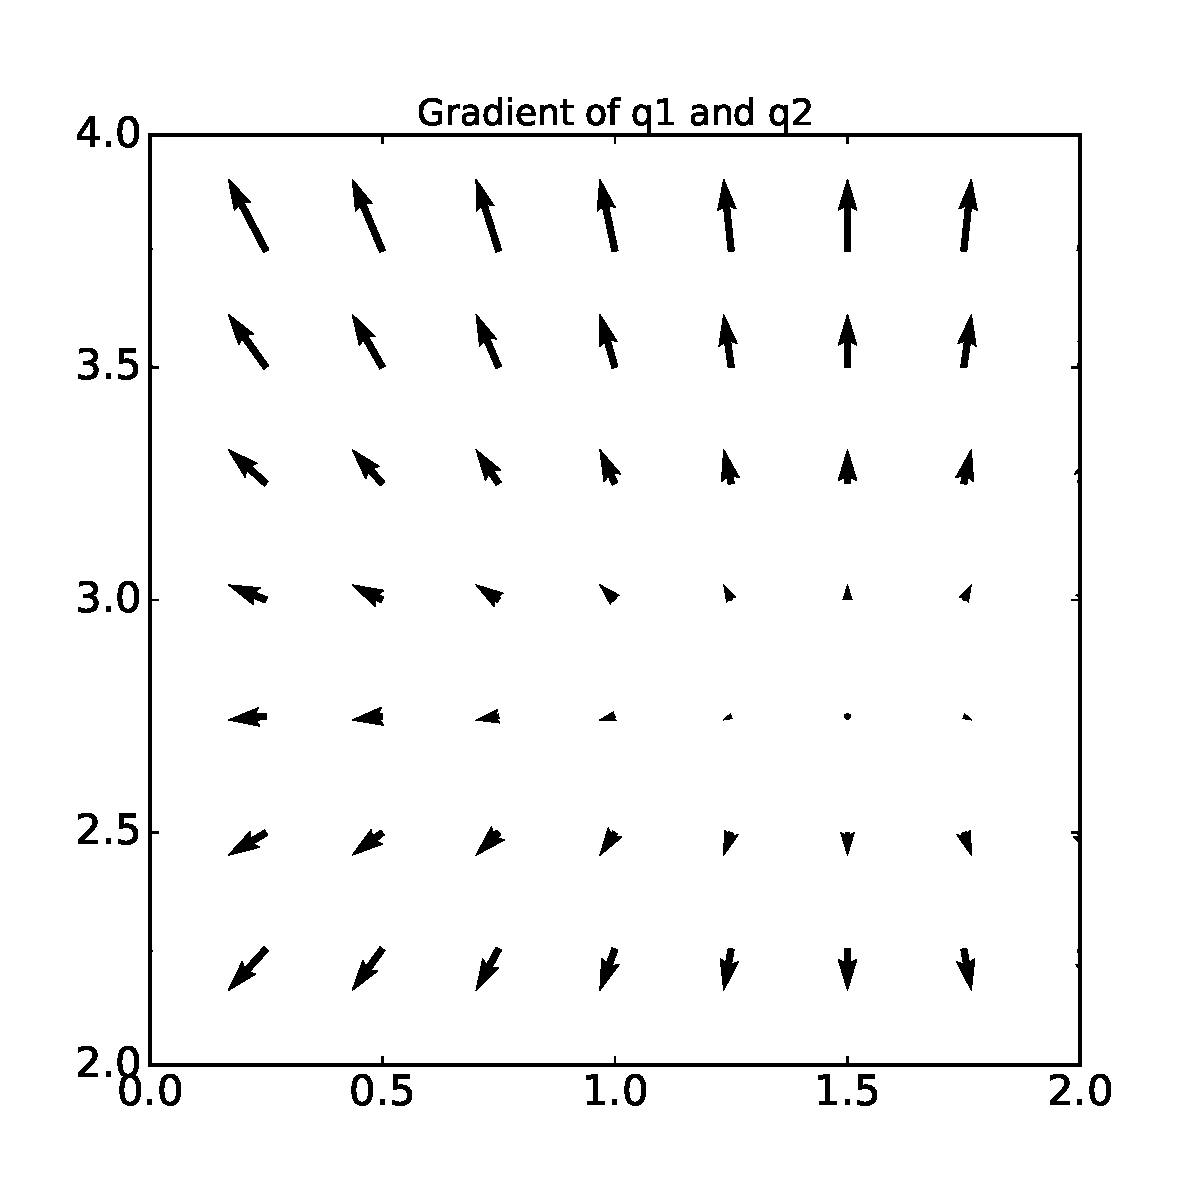
\includegraphics[width=\textwidth]{simple-linear-system/figures/gradient_2d_narrow_prior}
		\caption{Gradient with standard deviation $\sigma = 1$}
		\label{fig:linear_system.prior_influence.narrow}
	\end{subfigure}%
	\begin{subfigure}{.5\textwidth}
		\centering
		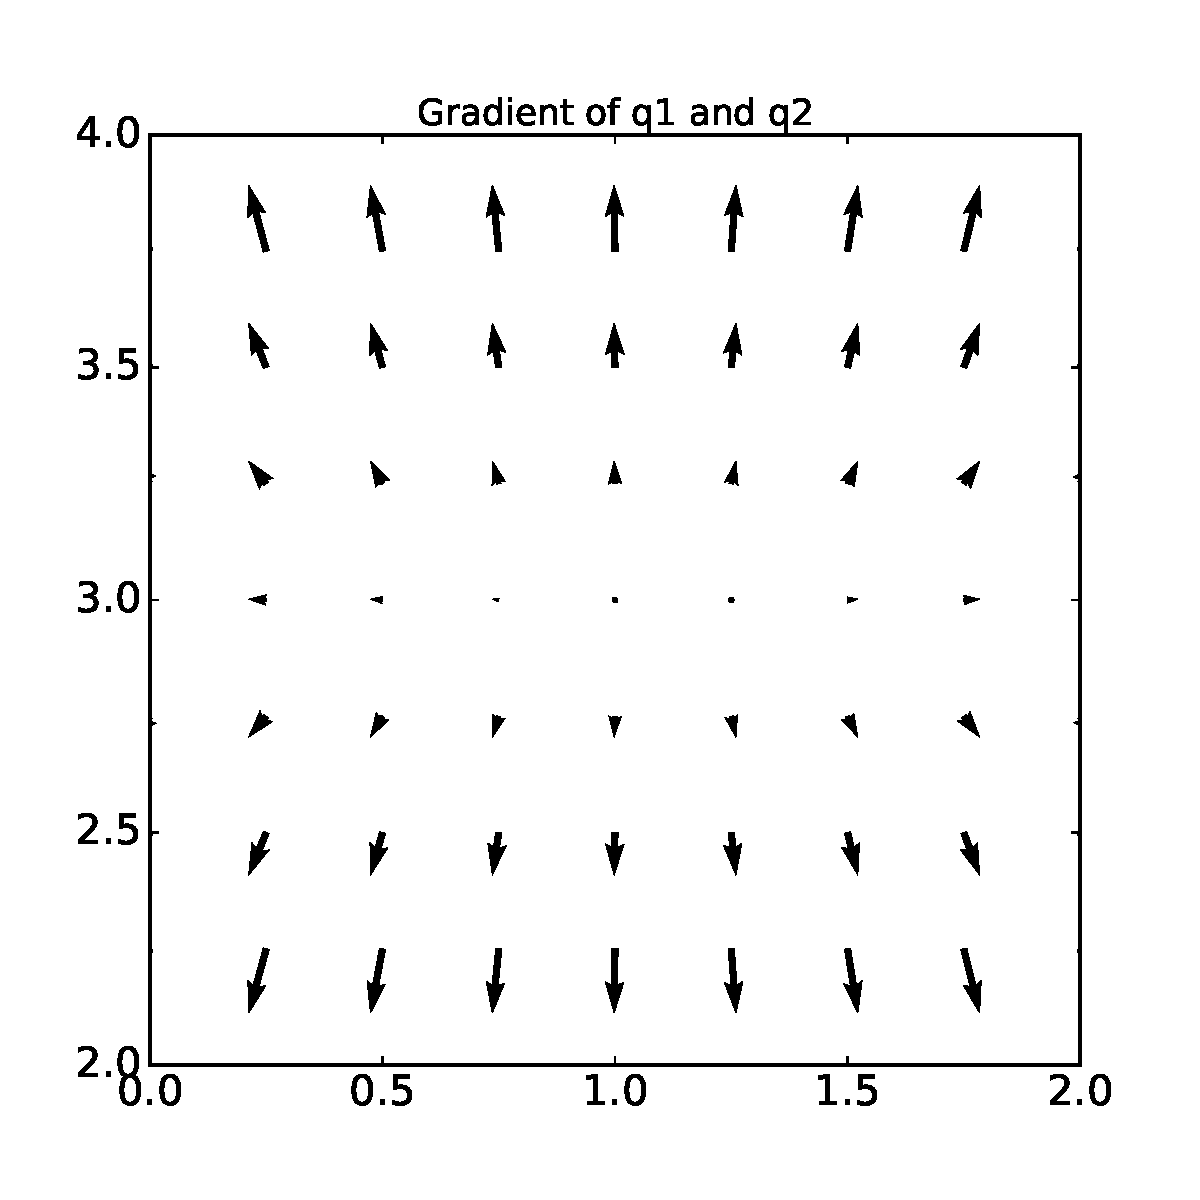
\includegraphics[width=\textwidth]{simple-linear-system/figures/gradient_2d_wide_prior}
		\caption{Gradient with standard deviation $\sigma = 5$}
		\label{fig:linear_system.prior_influence.wide}
	\end{subfigure}
	\caption{Normalized gradient of 2D misfit functionals with differently confined prior information. The means of the prior are for both parameters 2. It is obvious that decreasing the standard deviation for all parameters means that we increase the importance of the prior over the data, `pulling' the minimal gradient more towards the prior mean. Similar effects can be attained with increasing the magnitude of the data covariance matrix. Together, these matrices finely tune the minimum of the misfit function. Choosing well informed data and parameter covariace matrices is essential to meaningful \gls{HMC} sampling. In this example, the data covariance was uniformly 0.5.}
	\label{fig:linear_system.prior_influence}
\end{figure}

\index{Trajectories}For illustration purposes, 50 time steps were taken with a stepsize of 0.05 in time units (actual units of time might be a bit meaningless, without defining the units of length and mass). Using the unit mass matrix now generates trajectories like the one described in Figure~\ref{fig:linear_system.trajectory_simple}. 

\begin{figure}
	\centering

	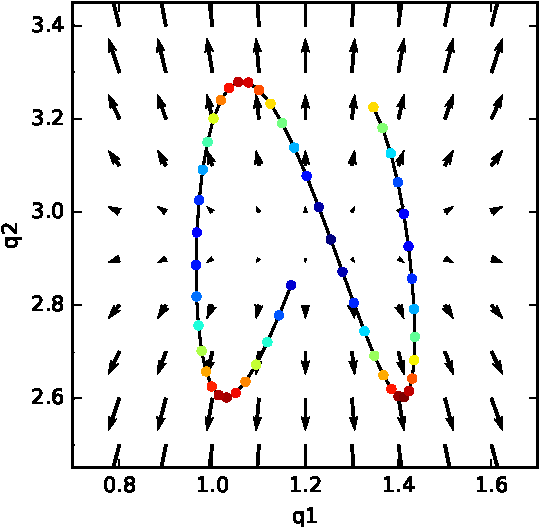
\includegraphics[width=0.5\textwidth]{simple-linear-system/figures/trajectory_simple}

	\caption{Untuned trajectory of the simple linear system described in Equation~\eqref{eq:linear_system.system}. The color of the trajectory points represents the normalized misfit, with red being the highest value, and dark blue being the lowest. Note that the direction of the trajectory can not be determined upon inspection of the trajectory itself; Hamilton's equation are invariant under time reversal. A particle would traverse exactly the same trajectory in reverse if at the end it's momentum would be reversed. The trajectory is superimposed on the gradient of the misfit functional $\chi$, which acts as the direction of the largest increase in gravitational potential. A particle starting without momentum would start to roll in opposite direction of these vectors, eventually orbiting the point of zero gradient (without energy loss it can never reach a steady state in the point of minimum energy).}
	\label{fig:linear_system.trajectory_simple}
\end{figure}	

\paragraph{Mass matrix optimization}\index{Mass matrix}\index{Trajectories!Tuning the}There are some undesirable characteristics of this trajectory. Due to the mass matrix being a diagonal unit matrix, but the misfit functional being elongated along the dimension of parameter $q_1$ the oscillations in either dimension do not have the same period. Using a mass matrix based on Equation~\eqref{eq:massMatrixForward} (which is still diagonal with the current forward model) will equalize oscillations. The reason this behavior is desired is that this way we see as many different energy levels in every dimension. The result of assigning the mass matrix based on the trace of $\MatrixVariable{G}^T\MatrixVariable{G}$ is seen in Figure~\ref{fig:linear_system.trajectory_massTuned}. The resulting mass matrix is ~
\begin{gather}\label{eq:linear_system.massMatrix}
\MatrixVariable{M} = 
\begin{pmatrix}
1 & 0\\
0 & 4\\
\end{pmatrix}.
\end{gather}

\begin{figure}
	\centering
	
	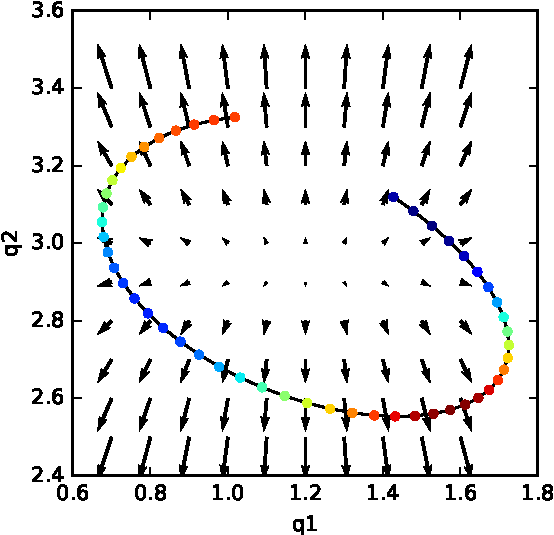
\includegraphics[width=0.5\textwidth]{simple-linear-system/figures/trajectory_massTuned}
	
	\caption{Trajectory tuned with mass matrix, according to the simple linear system described in Equation~\eqref{eq:linear_system.system}. The color of the trajectory points represents the normalized misfit, with red being the highest value, and dark blue being the lowest. With this augmented mass matrix, oscillations are equal in duration for each dimension.}
	\label{fig:linear_system.trajectory_massTuned}
\end{figure}

\paragraph{No U-Turn Criterion}\index{Trajectories!Trajectory length}\index{Trajectories!Tuning the}\index{No U-Turn Criterion}Visible now in Figure~\ref{fig:linear_system.trajectory_massTuned} is another characteristic of untuned trajectories. What would be ideal is that the algorithm explores the model space as efficiently as possible. The trajectory depicted in the figure traverses the model space around the minimum fully, but also start to come back to the original position. This so called `U-Turn' behavior can be mitigated by terminating the trajectory as soon as one detects the propagated model coming closer to the initial model. This point is reached as
\begin{gather}
	  \mathbf{v}(t) \cdot \left[ \mathbf{m}(t) - \mathbf{m}_0 \right] < 0, \quad
	 \text{and} \quad
	 \mathbf{v}_0\cdot \left[ \mathbf{m}_0 - \mathbf{m}(t) \right] < 0.
\end{gather}
This means that as soon as the momenta vectors for both the beginning and end of the trajectory both make an angle of less than 90 degrees with the vector connecting the points, so if the two models are `moving towards' each other, the trajectory is terminated. An illustration of a terminated trajectory is given in Figure~\ref{fig:linear_system.trajectory_uTurn}. By limiting the trajectories using this criterion, and additionally increasing the step size so only a few samples are needed to traverse to model space will effectively reduce computational costs of proposing new models.

\begin{figure}
	\centering
	
	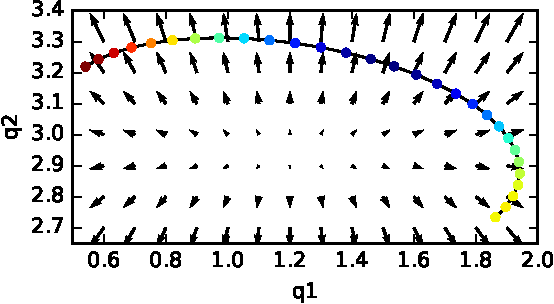
\includegraphics[width=0.5\textwidth]{simple-linear-system/figures/trajectory_uTurn_29_samples}
	
	\caption{Trajectory tuned with the \textbf{No U-Turn Criterion} and forward model based mass matrix. The color of the trajectory points represents the normalized misfit, with red being the highest value, and dark blue being the lowest. As soon as the momentum of the initial point and the last point of the trajectory point `towards' eachother the trajectory is terminated. In this case, 29 samples were made before the trajectory was terminated.}
	\label{fig:linear_system.trajectory_uTurn}
\end{figure}

\paragraph{Stepsize of the trajectories}\index{Trajectories!Tuning the}\index{Trajectories!Stepsize} The step size is another important tuning parameter. Wasting many computation on many steps is wasteful if the `particle' will end up in the same place, as was done in previous illustrations. According to \cite{neal2011mcmc} the maximum step size is defined by the minimum standard deviation of momentum, or square root of the mass matrix.

\paragraph{Results}




